% Generated by fb-detect.R from fb-detect.csv, then manually edited to
% ensure that the labels for the five labeled points do not overlap,
% give those points their own style in the legend, remove all
% clipping, adjust font and line sizes finely, clean up redundant or
% unnecessary drawing operations, and eliminate all use of opacity
% (partial opacity is not needed, and merely having /CA settings in
% the PDF can cause issues downstream).
%
% Most of the above adjustments are cosmetic, but the manual tuning of
% point labels is essential.
%
% If you modify this file, take care not to introduce any uncommented
% whitespace, _including newlines_, outside the tikzpicture environment;
% it can cause things to move around in the overall document.
%
% Created by tikzDevice version 0.6.2 on 2012-01-07 21:07:33
% !TEX encoding = UTF-8 Unicode
\beginpgfgraphicnamed{figures/fb-detect-c}%
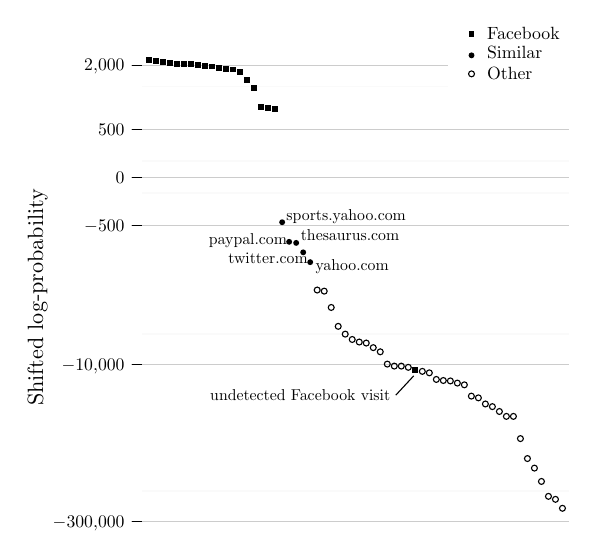
\begin{tikzpicture}[x=1pt,y=1pt]

% legend
\fill (168.31,199.48) rectangle	(170.44,201.62);
\fill (169.37,192.79) circle (  1.07);
\draw (169.37,186.10) circle (  1.07);

\begin{scope}[anchor=base west, inner sep=0pt, outer sep=0pt]
\node [scale=0.64] at (175,198.35) {Facebook};
\node [scale=0.64] at (175,191.52) {Similar};
\node [scale=0.64] at (175,183.89) {Other};
\end{scope}

% y-axis labels
\node[rotate=90,anchor=base,inner sep=0pt,outer sep=0pt,scale=0.8]
  at ( 14.54,105.39) {Shifted log-probability};

\begin{scope}[anchor=base east, inner sep=0pt, outer sep=0pt]
\node[scale=0.64] at ( 44, 22.05) {$-$300,000};
\node[scale=0.64] at ( 44, 79.06) {$-$10,000};
\node[scale=0.64] at ( 44,129.28) {$-$500};
\node[scale=0.64] at ( 44,146.60) {0};
\node[scale=0.64] at ( 44,163.93) {500};
\node[scale=0.64] at ( 44,187.17) {2,000};
\end{scope}

% y-ticks
\begin{scope}[line width=0.2pt, line cap=round]
\draw ( 46.68, 24.25) -- ( 50.30, 24.25);
\draw ( 46.68, 81.26) -- ( 50.30, 81.26);
\draw ( 46.68,131.48) -- ( 50.30,131.48);
\draw ( 46.68,148.81) -- ( 50.30,148.81);
\draw ( 46.68,166.14) -- ( 50.30,166.14);
\draw ( 46.68,189.37) -- ( 50.30,189.37);
\end{scope}

% y-grid
\definecolor[named]{gridminor}{gray}{0.98}
\definecolor[named]{gridmajor}{gray}{0.80}

\begin{scope}[color=gridminor, line width=0.6pt]
\draw ( 50.30, 35.32) -- (204.77, 35.32);
\draw ( 50.30, 92.07) -- (204.77, 92.07);
\draw ( 50.30,143.10) -- (204.77,143.10);
\draw ( 50.30,154.52) -- (204.77,154.52);
\draw ( 50.30,181.49) -- (160.77,181.49);
\end{scope}

\begin{scope}[color=gridmajor, line width=0.2pt]
\draw ( 50.30, 24.25) -- (204.77, 24.25);
\draw ( 50.30, 81.26) -- (204.77, 81.26);
\draw ( 50.30,131.48) -- (204.77,131.48);
\draw ( 50.30,148.81) -- (204.77,148.81);
\draw ( 50.30,166.14) -- (204.77,166.14);
\draw ( 50.30,189.37) -- (160.77,189.37);
\end{scope}

% data
\fill ( 51.76,189.97) rectangle ( 53.90,192.10);
\fill ( 54.29,189.73) rectangle ( 56.43,191.86);
\fill ( 56.83,189.16) rectangle ( 58.96,191.30);
\fill ( 59.36,189.00) rectangle ( 61.49,191.13);
\fill ( 61.89,188.72) rectangle ( 64.02,190.85);
\fill ( 64.42,188.60) rectangle ( 66.56,190.73);
\fill ( 66.96,188.48) rectangle ( 69.09,190.61);
\fill ( 69.49,188.27) rectangle ( 71.62,190.40);
\fill ( 72.02,187.74) rectangle ( 74.15,189.87);
\fill ( 74.55,187.71) rectangle ( 76.69,189.84);
\fill ( 77.08,187.26) rectangle ( 79.22,189.40);
\fill ( 79.62,186.66) rectangle ( 81.75,188.79);
\fill ( 82.15,186.60) rectangle ( 84.28,188.73);
\fill ( 84.68,185.71) rectangle ( 86.82,187.85);
\fill ( 87.21,182.98) rectangle ( 89.35,185.12);
\fill ( 89.75,179.87) rectangle ( 91.88,182.01);
\fill ( 92.28,173.20) rectangle ( 94.41,175.34);
\fill ( 94.81,172.65) rectangle ( 96.94,174.78);
\fill ( 97.34,172.34) rectangle ( 99.48,174.47);

\fill (147.99, 77.88) rectangle (150.12, 80.02);
\coordinate (fp) at (148.5, 77); % used below
\coordinate (fpl) at (142, 70);

\fill (100.94,132.49) circle (  1.07);
\fill (103.47,125.41) circle (  1.07);
\fill (106.01,125.02) circle (  1.07);
\fill (108.54,121.61) circle (  1.07);
\fill (111.07,118.06) circle (  1.07);

\draw (113.60,107.99) circle (  1.07);
\draw (116.14,107.59) circle (  1.07);
\draw (118.67,101.69) circle (  1.07);
\draw (121.20, 94.87) circle (  1.07);
\draw (123.73, 92.06) circle (  1.07);
\draw (126.26, 90.12) circle (  1.07);
\draw (128.80, 89.20) circle (  1.07);
\draw (131.33, 88.83) circle (  1.07);
\draw (133.86, 87.17) circle (  1.07);
\draw (136.39, 85.67) circle (  1.07);
\draw (138.93, 81.23) circle (  1.07);
\draw (141.46, 80.51) circle (  1.07);
\draw (143.99, 80.50) circle (  1.07);
\draw (146.52, 80.06) circle (  1.07);
\draw (151.59, 78.60) circle (  1.07);
\draw (154.12, 78.07) circle (  1.07);
\draw (156.65, 75.68) circle (  1.07);
\draw (159.18, 75.30) circle (  1.07);
\draw (161.72, 75.14) circle (  1.07);
\draw (164.25, 74.37) circle (  1.07);
\draw (166.78, 73.74) circle (  1.07);
\draw (169.31, 69.65) circle (  1.07);
\draw (171.85, 69.03) circle (  1.07);
\draw (174.38, 66.82) circle (  1.07);
\draw (176.91, 65.86) circle (  1.07);
\draw (179.44, 64.10) circle (  1.07);
\draw (181.97, 62.33) circle (  1.07);
\draw (184.51, 62.33) circle (  1.07);
\draw (187.04, 54.31) circle (  1.07);
\draw (189.57, 47.10) circle (  1.07);
\draw (192.10, 43.64) circle (  1.07);
\draw (194.64, 38.82) circle (  1.07);
\draw (197.17, 33.44) circle (  1.07);
\draw (199.70, 32.36) circle (  1.07);
\draw (202.23, 29.12) circle (  1.07);

% point labels
\begin{scope}[anchor=base west, inner sep=0pt, outer sep=0pt]
\node [scale=0.57] at (102.5,133) {sports.yahoo.com};
\node [scale=0.57] at (74.5,124.5) {paypal.com};
\node [scale=0.57] at (107.7,126) {thesaurus.com};
\node [scale=0.57] at (81.5,117.5) {twitter.com};
\node [scale=0.57] at (113,115) {yahoo.com};
\end{scope}

\draw (fp) -- (fpl);
\node [anchor=east, scale=0.57] at (fpl) {undetected Facebook visit};

\end{tikzpicture}\endpgfgraphicnamed%
